%% PART 2 : SERIOUS GAMES
\subsection{Serious Games}
Les serious games ou jeux sérieux sont donc une catégorie de jeux ayant la particularité d'avoir une portée supplémentaire au divertissement. Ils restent cependant des jeux en ce qu'ils en intégrent les caractéristiques ludiques, et même plus les utilisent pour parvenir plus aisément ou efficacement à leur objectif sérieux. Dans cette partie, nous allons voir comment un jeu sérieux  peut parvenir à des résultats sérieux et quels sont les mécanismes sous-jacents qui permettent une telle efficacité, souvent inconsciente chez le joueur.
	%% A Serious Games et Théories Comportementales 
	\subsubsection{Serious Games et Théories Comportementales }
			\paragraph{}
Les jeux vidéo sérieux se présentent comme un potentiel médiateur dans la modification des habitudes comportementales en permettant d’inclure des connaissances pratiques dans un modèle ludique apprécié. Il est possible d’y mettre en place des procédures de changement comme l’établissement d’objectifs ou la modélisation et le développement de compétences dans un environnement attrayant, significatif et immersif [Baranowski et al, 2008]\cite{Bara08}. \\
Les jeux vidéo promeuvent les interactions sociales et d’apprentissage [Wideman et all, 2008], créent un environnement où les actions du joueur ont un effet [Gee, 2004]\cite{Gee04} , encouragent la résolution de problèmes [Gee, 2004]\cite{Gee04} et renforcent la compréhension en créant des situations de réflexion ou en aidant le joueur dans ses objectifs [Gee, 2004]\cite{Gee04}. Enfin, les jeux sérieux pour la santé sont fait pour distraire le joueur tout en l’éduquant, en l’entrainant ou en changeant ses comportements [Stokes, 2005]\cite{Stok05}.

		\subsubsection*{Théories comportementales}
Le comportement est la résultante d’influences multiples, rendant ainsi souvent les personnes réfractaires au changement [Baranowski, Lin \& al, 1997]\cite{Bara97}. Le comportement doit alors être considéré comme un mécanisme complexe découlant de l’enchaînement de plusieurs étapes. Ainsi, plutôt que de chercher à impacter directement le comportement, les experts comportementaux valorisent une action sur ces facteurs intermédiaires, appelés médiateurs. Changer ces médiateurs permet de changer le comportement [Baranowski, Lin \& al 1997]\cite{Bara97}.
\paragraph{}Plusieurs grandes théories comportementales existent~:
\begin{itemize}
	\item la théorie d’inoculation comportementale [McGuire, 1961]
	\item la théorie socio-cognitive [Bandura, 1986]
	\item la théorie de l’auto-détermination [Ryan \& Deci, 2000]
	\item la théorie de l’immersion [Green \& Brock, 2000]
\end{itemize}

\paragraph{}De ces théories, l’on peut alors identifier un certains nombre de ces facteurs médiateurs tels que : l’immersion, l’attention, l’auto-régulation, le développement de compétences, la motivation interne et externe, l’autonomie ou encore le sentiment de compétence. La science du comportement fournit aussi des techniques qui facilitent le changement comportemental, et propose d’utiliser ces facteurs dans les média de divertissement tel que le jeu vidéo.\\
Le modèle : "Elaboration Likelihood Model" [Petty \& Cacioppo, 1986] soutient ainsi que des personnages crédibles, attrayants et sympathiques sont plus susceptibles d’être persuasifs que les autres et peuvent donc servir d’intermédiaires pour véhiculer un message. \\
La théorie d’inoculation comportementale [McGuire, 1961] met en garde contre une possible contre-productivité en identifiant et en réfutant les menaces potentielles à l’accomplissement des objectifs du changement désiré.\\
La théorie socio-cognitive [Bandura, 1986] préconise l’établissement d’objectifs et le développement de compétences comme paramètres importants dans le changement comportemental.\\
Enfin, les théories socio-cognitive [Bandura, 1986] et d’auto-détermination [Ryan \& Deci, 2000] mettent toutes deux l’accent sur l’importance du feedback pour guider et mettre en forme le comportement durant le processus de changement.	

		\subsubsection*{Théories comportementales dans un serious game éducatif}
			\paragraph{Identification \\ \quad}
Fait référence aux feedbacks ou aux conseils qui sont \emph{personnalisés} afin de mieux toucher le joueur [Kreuter, Strecher \& Glassman, 1999]. 
			\paragraph{Mini-jeux de connaissances \\ \quad}
Des connaissances pratiques et théoriques spécifiques sont un élément nécessaire, mais pas suffisant, d’une modification des habitudes comportementales [Bandura, 1986]. Ces mini-jeux peuvent être explicites (dans un mode à part) ou correspondrent aux boucles micro du gameplay.
			\paragraph{Ajustement des objectifs \\ \quad}
C’est un processus complexe qui permet à la fois de définir un objectif et les manières de l’atteindre [Gollwitzer, 1999], en prenant en considération les capacités et valeurs personnelles pour les lier à son objectif [Ryan \& Deci, 2000]. Parce que l’autonomie améliore la motivation personnelle [Ryan \& Deci, 2000], proposer et permettre au joueur de réaliser ses propres choix ou de paramétrer ses objectifs est donc conseillé.
			\paragraph{Résolution de problèmes \\ \quad}
Bien que les difficultés et obstacles interfèrent de premier abord dans la réalisation de ses objectifs, arriver à les surmonter est un moteur de motivation puissant [Frauenknecht \& Black, 1995]. Le joueur doit prévoir ces difficultés et mettre en place un plan pour arriver à les dépasser. Ces solutions doivent paraitre réalisables et plausibles pour ne pas décourager le joueur [Elaboration Likelihood Model : Petty \& Cacioppo, 1986].
			\paragraph{Exposition des motivations \\ \quad}
La théorie de l’auto-détermination [Ryan \& Deci, 2000] indique que la motivation personnelle est d’autant plus importante que la personne voit le lien entre son comportement et des choses importantes pour elle, comme une valeur qui lui est chère. Par exemple dans un serious game de rééducation motrice, si pouvoir faire du tennis est une chose importante pour le joueur-patient, on lui rappellera que réaliser des étirements quotidient permet de récupérer plus rapidement.
			\paragraph{Revue des objectifs et du travail accompli\\ \quad}
Cette activité renforce le sentiment d’accomplissement personnel et augmente l’auto-efficacité [Bandura, 1986].
			\paragraph{Feedback \\ \quad}
Un feedback bien conçu renforce l’efficacité personnelle [Schuk, 1986] et le sentiment de compétence. [Ryan \& Deci, 2000]
			
\paragraph{}
Pour vérifier l'application de ces théories sur un cas pratique, [Thompson et al, 09] ont participé à la création d'un Serious Game~: DIAB. DIAB est un jeu vidéo divertissant, mais sérieux et se basant sur ces concepts théoriques, conçu pour réduire les risques de diabète de type 2 et d’obésité infantile. Il émerge de cette expérience que les jeux sérieux fondés sur une base théorique peuvent être efficaces pour parvenir à un changement à la fois dans le régime alimentaire et l’activité physique. Peu est encore connu dans le domaine, mais il en sort que les mécanismes et processus de changements comportementaux ont aussi leur place dans les jeux sérieux et peuvent permettre d'améliorer l'efficacité de ces derniers. Cette expérience décrit aussi comment des experts du divertissement et d'une spécialité différente peuvent allier leurs talents respectifs pour créer un jeu sérieux efficace et divertissant basé sur un socle théorique. 
	%% Apprentissage et propriétés des jeux vidéo
	\subsubsection{Apprentissage et propriétés des jeux vidéo}
			\subsubsection*{Théories de l'apprentissage}
Les serious games sont aujourd'hui utilisés comme nouveaux vecteurs d'apprentissage. Ils sont en effet porteurs de nombreux éléments qui sont propices à l'apprentissage [Baranowski, 08]. On ne connait cependant pas la relation entre les attributs d'un jeux et les résultats de l'apprentissage, ni si ces liens sont directs ou indirects, si un seul paramètre ou une combinaison de ceux-ci auront un impact différent ou plus important [Wilson 09]\cite{Wils09}. 

\paragraph{}Plusieurs théories de l'apprentissage permettent d'en expliquer les mécanismes, que nous essaieront par la suite de lier aux paramètres d'un jeu vidéo.\\

\emph{Cognitive learning outcomes} :  Dans cette théorie, [Kraiger et all, 93] développent 3 notions : la connaissance déclarative (le quoi), la connaissance procédurale (le comment) et le savoir tacite ou stratégique (qui, quand, pourquoi). Ces trois catégories décrivent le processus cognitif d'apprentissage, et se rapprochent fortement des sous-catégories de la connaissance de [Bloom, 1956].\\ 

\emph{Skill-based learning outcomes} : En poursuivant le développement de leurs capacités cognitives, les apprenants progressent vers des méthodes d'apprentissage basées sur les compétences. Ces compétences se concentrent sur le développement de techniques ou de compétences motrices en dépassant progressivement la phase de réflexion consciente. Les compétences psychomotrices demandent de la pratique et peuvent être catégorisées parmi 7 catégories de la plus simple à la plus complexe : perception (sentir les moteurs permettant de réaliser le mouvement), volonté d'agir, imitation (être capable de réaliser un mouvement défini), automatisme(réalisation d'un schéma moteur), réponse manifeste complexe, adaptation et originalité.\\ 

\emph{Affective learning outcomes} [Kraiger et al 1993]. Selon cette théorie, l'apprentissage façonne aussi les sentiments d'un individu. Kraiger et al décrivent les résultats d'un apprentissage par les émotions comme impliquant des concepts tels que l'attitude, la motivation et les objectifs.\\

En 2012, Curtiss s'inspire des lois de l'apprentissage de Thorndike qui décrivent trois principes : la bonne volonté(readiness), la pratique(exercice) et l'effet(effect), auxquels ont été depuis ajoutées les lois de primauté, d'intensité et de récense. Son travail portant sur l'utilisation de serious games éducatifs dans l'armée, il simplifie et ne garde de ces lois que les aspects inconditionnels, dans le temps ou le milieu d'apprentissage par exemple. Il décrit ainsi six nouvelles lois de l'apprentissage pour les jeux, décrites dans le tableau de la figure \ref{laws_of_learning_for_games}.

\begin{figure}[h!]
	%\centering
	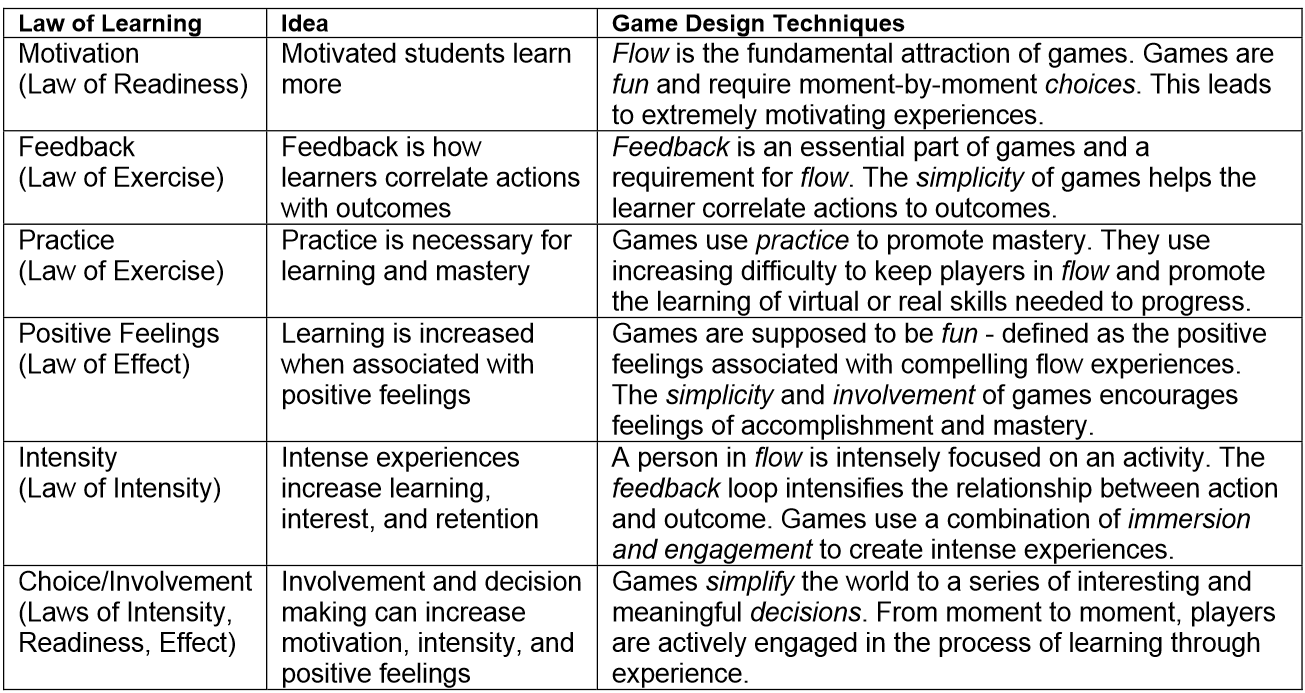
\includegraphics[width=1.1\linewidth]{images/laws_of_learning_for_games.png}
	\caption{Lois de l'apprentissage dans les jeux vidéo, [Murphy, 2011]\cite{Murp11}}
	\label{laws_of_learning_for_games}
\end{figure}

			\subsubsection*{Propriétés des jeux vidéo}
En 1984, [Driskell and Dwyer]\cite{Dris84}réalisent un premier état de l'art et trouvent que plusieurs caractéristiques des jeux vidéo peuvent influer sur les propriétés d'apprentissage et de motivation : des objectifs spécifiques, un challenge, de la fantaisie et du mystère. Ils théorisent qu'une augmentation de la motivation produit une augmentation de l'attention et mène à une meilleure mémorisation des acquis (connaissance déclarative) et une focalisation de l'attention (stratégie cognitive).\newline
[Malone et Lepper, 1987] mentionnent le challenge, la curiosité, le contrôle et la fantaisie comme caractéristiques intégrantes des jeux vidéo. Selon [de Felix et Johnson , 1993], les jeux sont composés d'éléments visuels dynamiques, d'interactions, de règles et d'objectifs. Puis [Thiagarajan, 1999] affirme que le conflit, le contrôle, la terminalité et l'artifice sont les quatre éléments nécessaires d'un jeu. En 2001, [Garis and Ahlers, 01] donnent 39 descripteurs qui seront réduits à 12 pour ne garder que les paramètres statistiquement les plus significatifs pour renforcer la sensation de "game-like". \\ Finalement en 2002, [Garris et al] proposent un sous-ensemble de tous ces attributs qui seront considérés commes les paramètres de jeu clefs de l'apprentissage~:
\begin{itemize}
	\item la fantaisie
	\item les règles
	\item la stimulation sensorielle
	\item le challenge
	\item le mystère
	\item le contrôle
\end{itemize}

\paragraph{}En 2009, [Wilson et al]\cite{Wils09} partent de l'ensemble de paramètres de [Garris et al] pour enrichir le modèle avec de nouveaux paramètres qui leur semblent avoir un impact sur l'apprentissage.
Les tableaux \ref{game_attributes_one} et \ref{game_attributes_two} indiquent et décrivent ces douze attributs.

\begin{figure}[h!]
	\centering
	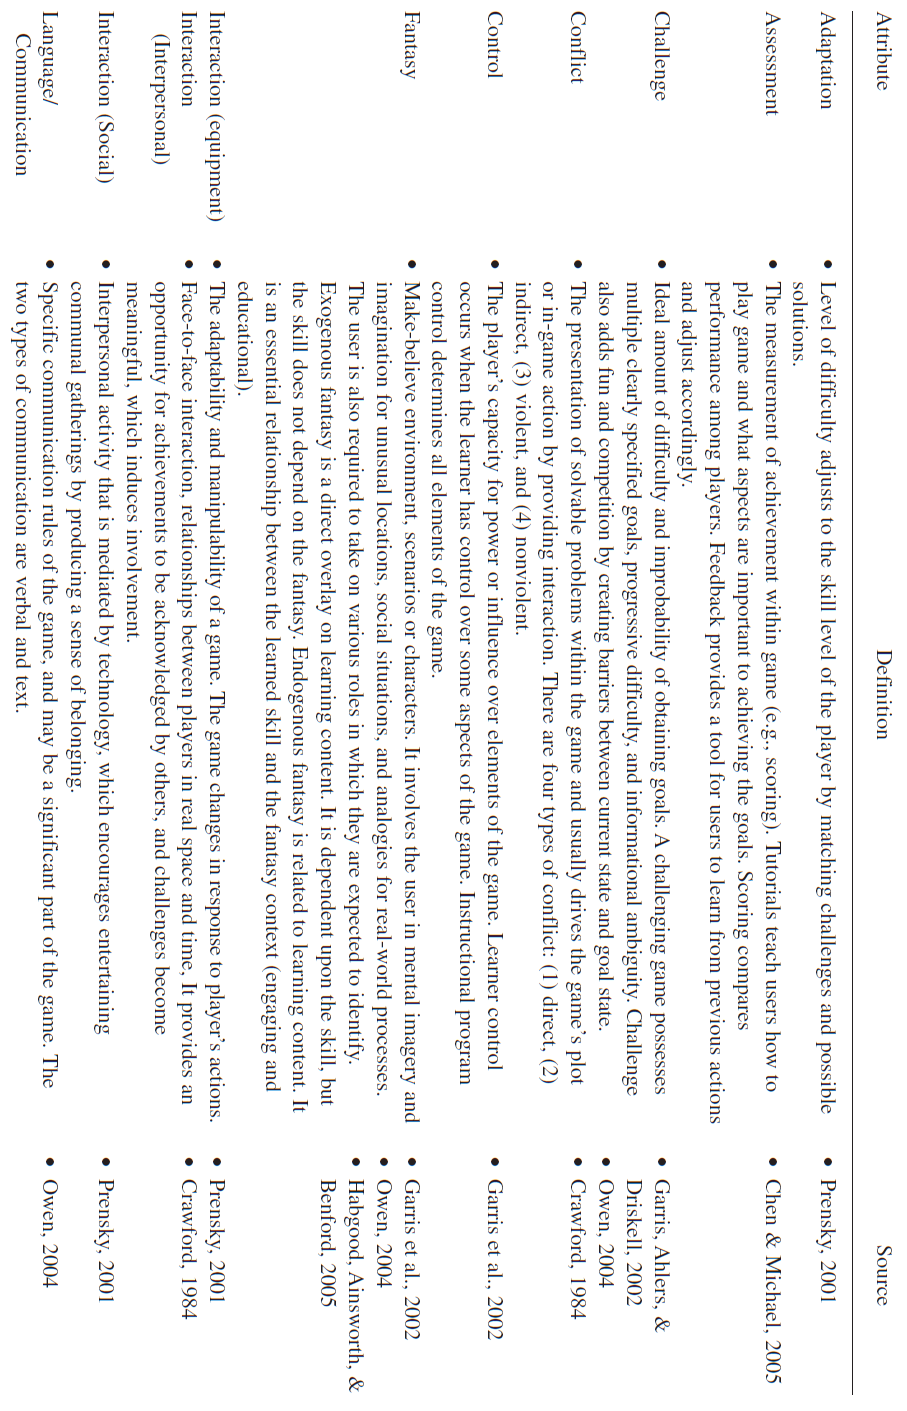
\includegraphics[width=\linewidth, height=\textheight ]{images/game_attributes_one}
	\caption{Propriétés des jeux vidéo et leur définition. (1/2) \cite{Wils09}}
	\label{game_attributes_one}
\end{figure}
\begin{figure}[h!]
	\centering
	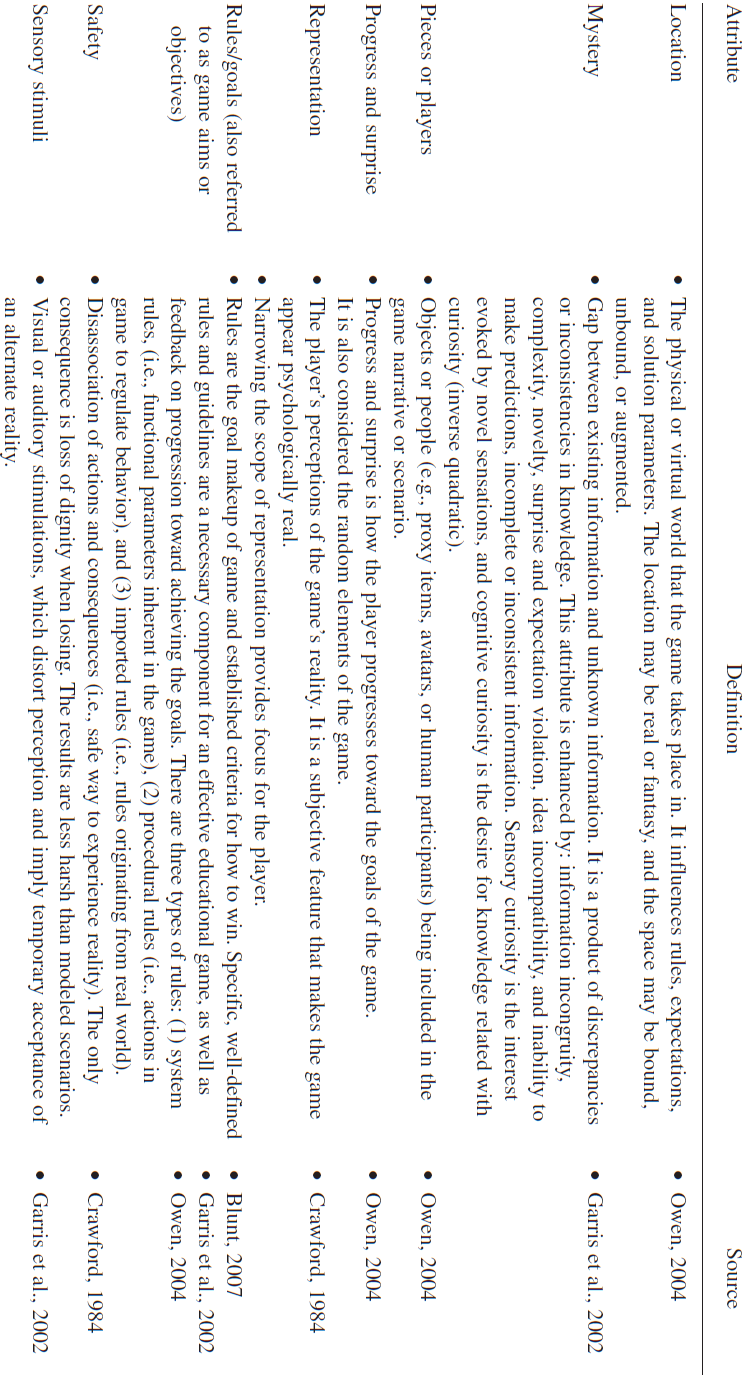
\includegraphics[width=\linewidth, height=\textheight ]{images/game_attributes_two}
	\caption{Propriétés des jeux vidéo et leur définition. (2/2) \cite{Wils09}}
	\label{game_attributes_two}
\end{figure}

		\subsubsection*{Les jeux vidéo comme outil d'apprentissage}
Les concepteurs de bons jeux vidéo mettent en place d'exellentes méthodes pour que les joueurs apprennent et aiment apprendre dans le jeu vidéo. Initialement, cet apprentissage ne concernent que les principes importants pour jouer au jeu, mais on observe très vite un phénomène d'apprentissage tangentiel chez les joueurs, qui apprennent aussi plus facilement des notions facultatives pour le gameplay. Gee se propose en 2005 de discuter de 13 principes d'apprentissage efficaces, et de leur intérêt à les mettre en application au travers de jeux vidéo. Il divises ces principes en trois catégories en précisant que le principal problème à la mise en place de tels systèmes d'apprentissage reste le coût.
			\paragraph{\emph{La participation des apprenants ( Empowered Learners)}}
			\begin{itemize}
				\item {Co-design} : l'apprenant doit être un acteur actif (producer) et non passif (consumer)
				\item {Customisation} : l'apprenant doit pouvoir prendre des décisions quant à la méthode
d'apprentissage (chacun est différent) et s'essayer (être encouragé) à de nouvelles.
				\item {Identification} : un apprentissage en profondeur requiert une réelle implication,
implication qui se fait bien plus présente lors d'un jeu de rôle
				\item {Manipulation et connaissance distribuée} : les sciences cognitives montrent que la
pratique, notamment au travers d'un tiers (robot, entité, etc) permet de ressentir soi
même les choses et de mieux les comprendre (empathie).
			\end{itemize}

			\paragraph{\emph{Résolution de problèmes}}
			\begin{itemize}
				\item {Difficulté progressive (well-ordered problems)} : être confronté trop tôt à un problème
trop difficile n'est pas efficace, bien que pouvant amener à des solutions très créatrices ;
alors qu'une évolution progressive de la difficulté permet à l'apprenant de comprendre seul au fur et à mesure.
				\item {Frustration plaisante} : notion de challenge : dur mais faisable.
				\item {Cycle d'expertise} : répéter et pratiquer ses compétences jusqu'à les maîtriser, puis
confronter l'apprenant à une difficulté lui demandant de mettre en pratique toute cette maîtrise, ancienne ou récente. Puis répéter ce cycle à un niveau plus élevé (système levels /boss).
				\item {Information ‘On Demand’ and ‘Just in Time’} :
On part du constat que les humains ne peuvent / veulent pas emmagasiner une grande quantité d'information sans contexte. On apprend beaucoup mieux une information si elle est donnée dans un cas d'utilisation, un contexte, liée à une image, etc. C'est le « just in time ». De la même manière, on peut vouloir la retrouver aisément lorsqu'on en a
besoin, le « on demand ». Cela se traduit dans les jeux par les tutoriels et manuels d'utilisation.
				\item {Aquarium} : C'est le principe de l'écosystème simplifié permettant d'appréhender un sous
ensemble des paramètres, afin de ne pas être directement surchargé par la masse d'information. Dans les jeux, on va penser aux démo ou aux ou premiers niveaux simplifiés (didacticiels).
				\item {Sandboxes : ou Bac à sable} : proposer un environnement identique à l'environnement
réel, mais plus sur et sécurisé. Dans ce contexte, l'apprenant va pouvoir expérimenter sans risque avec un réel sentiment d'accomplissement et d'authenticité. Il n'y a rien de pire qu'un jeu où après bien des efforts, on perd juste avant de pouvoir
sauver. Cela induit une manière de jouer très 'safe' où ne prend plus aucun risque sans chercher à explorer les possibilités du jeu.
				\item {Skills as Strategies} : Sur le principe de « c'est en forgeant que l'on devient forgeron »,
c'est à force de pratiquer une compétence que l'on finit par la maîtriser. Mais l'on n'aime pas pratiquer sans raison, il faut donc arriver à lier ses objectif personnels avec l'utilisation de la compétence. En jeu, passer par une phase obligatoire d'utilisation d'un skill (\emph{Zelda}).
		\end{itemize}
			\paragraph{\emph{Compréhension}}
		\begin{itemize}
				\item {Pensée globale (System Thinking)}: Comprendre comment s'intègre la notion ou compétence nouvelle dans le système global permet de mieux l'appréhender. Pousser cette compréhension (en montrant quels leviers d'action permet ou non chaque élément)de manière à être capable d'inférer les règles 'sémantiquement' liées.
				\item {Meaning as Action Image} : Le fait que quand les gens pensent à un concept, ils n'y
pensent pas à travers sa définition générale, mais à travers l'expérience personnelle qu'ils ont de ce concept. Lié au principe « Just on time and on demand».
		\end{itemize}	

	%% Serious games thérapeutiques
	\subsubsection{Serious games pour la santé TODO}
TODO 
\begin{figure}
TODO Succinte explication du lien entre mes composantes. Vérifier que ca se trouve avec le reste et pas en fin de document.
	\centering
	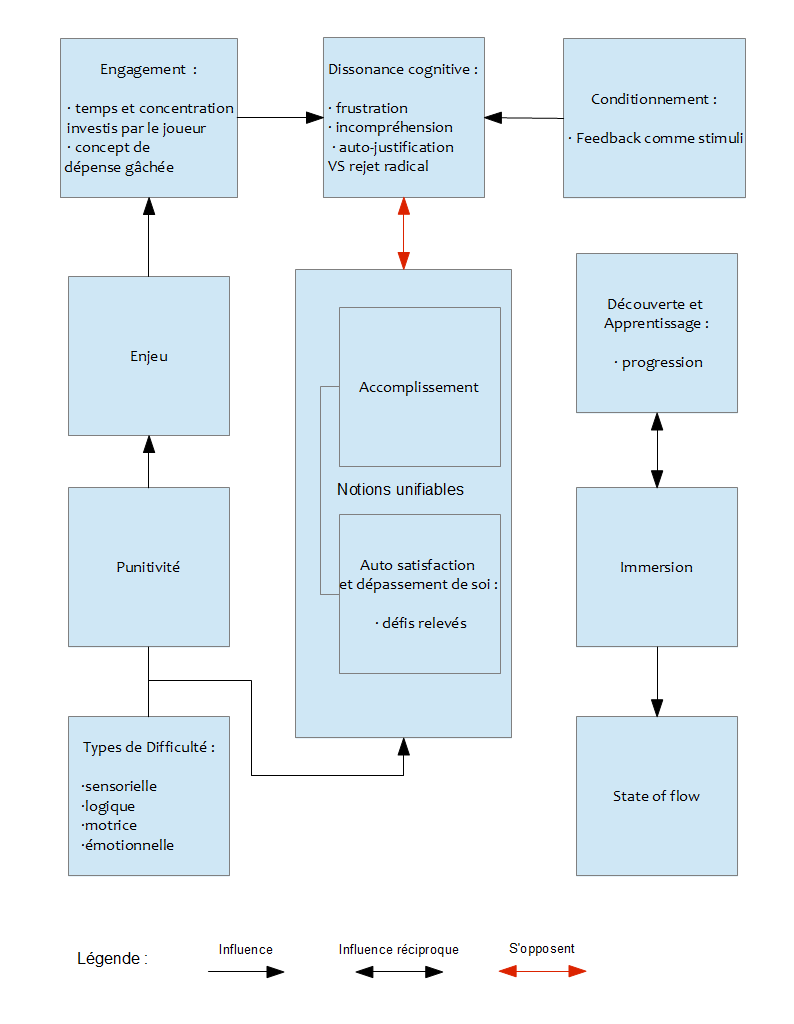
\includegraphics[height=19.6cm]{images/lien_theories}
	\caption{Relation entre les principaux ressorts psychologiques d'un jeu vidéo}
	\label{lien_theories}
\end{figure}